\chapter{Języki i technologie webowe}
\PartialToc
%\startcontents[chapters]
%\printcontents[chapters]{}{1}{\section*{\contentsname}}


\vspace{0.4cm}
\noindent
%%%%%%%%%%%% MAGDA :) %%%%%%%%%%%%
\answer{Zaznacz prawdziwe stwierdzenia. Droga pakietu w sieci Internet pomiędzy dwoma węzłami, tj. lista adresów węzłów odwiedzanych przez pakiet...}
{Zależy od dynamicznego routingu}
{T}
{Patrz poniżej}
{\\}
\noindent
Krótkie opowiadanie o rutowaniu.\\

Routing jest to należący do warsty 3 proces kierowania pakietów IP poprzez sieć tak, aby osiągneły one swój 
docelowy węzeł (identyfikowany poprzez Adres IP).\\
Router jako urządzenie odpowiedzialne za proces routingu odbiera pakiety IP i decyduje o tym, dokąd (na który podłączony do niego fizycznie interfejs, a) zostaną przesłane. Owy pakiet IP zawiera w sobie m.in. informację o odbiorcy (adres IP węzła docelowego) oraz wartość TTL (ang. Time To Live) bądącą liczbą przeskoków jaką jest w stanie stolerować pakiet przed uznaniem go za zaginiony. Router do wykonania swojego zadania posługuje się tablicą rutowania, w której to zapisane ma dokąd przesłać pakiet o danej adresacji. Zawartość owej tablicy rutowania jest wynikiem pracy protokołów rutowania (nie mylić z rutowalnymi/rutowanymi), które to dziela się na statyczne i dynamiczne.\\
Rutowanie statyczne polega na uzupełnieniu tablicy rutowania przez administratora. W takiej sytuacji rutery zawsze wybierają dla pakietu tę drogę, którą nakazał im administrator i w razie awarii części sieci nie mogą samodzielnie wybrać innej. W przypadku rutowania dynamicznego,  rutery samodzielnie zbierają informacje (np odległość do celu, przepustowość łącza, obciążenie łącza, koszt łącza) i aktualizują zapisy w tablicy; w razie tłoku lub awarii ruter sam decyduje o wybraniu dla pakietu alternatywnej drogi. 

W ten sposób pakiet danych przechodzi pomiędzy kolejnymi sieciami. Takie kolejne przejście
nazywane jest przeskokiem lub hop-em. W tym rozumieniu tablica rutingu zawarta w ruterze lub w
komputerze sieciowym zawiera właśnie przyporządkowania adresów IP dotyczące jednego hopu.\\
Równolegle do protokołu IP w warstwie 3 działa jego rozszerzenie ICMP – Internet Control Message Protocol. Stworzone zostało ono do celów diagnostyki połączeń IP oraz routingu. ICMP posługuje się komunikatami typu “Żyjesz? Żyję”, jak również rozsyłaniem informacji o przekroczeniu czasu życia pakietu na podstawie wartości TTL. ICMP jest więc prawa ręką wszystkich dynamicznym protokołów rutowania.\\ \\


Wnioski i zdania prawdziwe dla "drogi pakietu w sieci Internet pomiędzy dwoma węzłami":
\begin{itemize}
\item Droga pakietu jest bespośrednim efektem procesu rutowania; nie jest jednak zapamiętywana 
\item Długość tej drogi jest liczbą przeskoków pakietu, gdzie przeskokiem jest każdy router, przez który musi zostać przesłany pakiet aby osiągnąć swoją destynację.
\item W przypadku rutowania statycznego droga pakietu z A do B będzie zawsze taka sama
\item W przypadku rutowania dynamicznego droga pakietu z A do B może sie zmieniać - algorytm wybranego protokołu może zaproponowac inną, bardziej optymalną drogę na skutek zmian obciążenia sieci lub powstania ustarek
\item Podczas rutingu przekazanie pakietu do kolejnego węzła jest zawsze równoważne zmniejszeniu o 1 (jeden) wartości jego TTL (dokładniej: wartość TTL pakietu jest zmiejszana przez kolejny ruter, który został jego odbiorcą)
\item Jedną z metod sprawdzenia przemirzanej przez pakiet drogi z A do B jest zastosowanie narzędzia traceroute; traceroute działa na zasadzie rozsyłania pakietów zaadresowanych na B i przydzielaniu im różnym TTL, a następnie wyciagania wniosków z powracającyh komunikatów ICMP.
\end{itemize}


\vspace{0.4cm}
\noindent
Poprzedni opis: \\
Droga takiego pakietu zależy od stanu tablic routingu. Jeżeli stosowany jest routing dynamiczny wtedy pierwsza próba wysłania pakietu się nie powiedzie - router nie zna adresu mac celu i musi go odnaleźć w związku z czym porzuca pakiet, natomiast jeśli w tablicy routingu znajduje się już adres mac węzła docelowego pakiet pójdzie dalej. Całość oczywiście zależy od stopnia skomplikowania sieci (np. ilość routerów po drodze).
\\
\\
Ścieżka pakietu w prostej sieci jest bardzo fajnie i obrazowo opisana tutaj:\\
http://jaredheinrichs.com/tracing-packet-flow-between-a-2-switches-and-a-router.html



\vspace{0.4cm}
\noindent 
%%%%%%%%%%%% MAGDA :) %%%%%%%%%%%%
\answer{Serwery DNS oferują:}
{Translację nazw symbolicznych adresów poczty elektronicznej do nazw symbolicznych węzłów obsługujących te adresy}
{T}
{Patrz poniżej}
{Serwery DNS są między innymi odpowiedzialne za przechowywanie informacji specyficznych dla systemu dostarczania poczty, nazywanych rekordami MX. Rekord MX (ang. Mail eXchanger) precyzuje który host (lub grupa hostów) odbiera pocztę dla poszczególnych domen. Jeżeli nasza domena nie zawiera rekordu MX w systemie DNS przesyłki będą dostarczane bezpośrednio do naszego hosta, pod warunkiem że nasz host posiada w systemie DNS rekord A odzwierciedlający nazwę naszego hosta na odpowiadający jej numer IP. \\

Serwery DNS (Domain Name System) są znane głównie z translacji nazw symbolicznych na adresy IP oraz translacji odwrotnej (Reverse Lookup). Zawarte jednak pola w rekordach odpowiedzi DNS niosą dodatkowe informacje, co oznacza, że serwery DNS mogą mieć w swojej ofercie nieco więcej niż wspomniano powyżej.\\}

\vspace{0.4cm}
Najważniejsze typy rekordów DNS oraz ich znaczenie względem treści pytania:
\begin{description}
\item[A] adres hosta (ipV4) - translacja na adres IP
\item[AAAA]  adres hosta (ipV6) 
\item[PTR]  	
	rekord wskaźnika - mapuje adres IPv4 lub IPv6 na nazwę kanoniczną hosta. 		Określenie rekordu PTR dla nazwy hosta (ang. hostname) w domenie in-addr.arpa 	(IPv4), bądź ip6.arpa (IPv6), który odpowiada adresowi IP, pozwala na 			implementację odwrotnej translacji adresów DNS (ang. reverse DNS lookup) 
\item[MX] mapuje nazwę domeny DNS na nazwę serwera poczty oraz jego priorytet 
\item[CNAME]	alias nazwy domeny. Wszystkie wpisy DNS oraz poddomeny są 	poprawne także dla aliasu 
\item[TXT]	rekord ten pozwala dołączyć dowolny tekst do rekordu DNS 
\item[NS] Name Server, serwer nazw dla danej strefy 
\item[SOA]    rekord adresu startowego uwierzytelnienia (ang. start of authority record) ustala serwer DNS dostarczający autorytatywne informacje o domenie internetowej 
\end{description}


Narzędzia do odpytywania DSN (poza niewidocznym modułem przeglądarki): host, dig\\




\vspace{0.4cm}
\noindent 
%%%%%%%%%%%% MAGDA :) %%%%%%%%%%%%
\answer{Zaznacz prawdziwe stwierdzenie. Protokół HTTP w wersji 1.1...}
{Umożliwia transmisję danych nieprzekraczających 2kB}
{F}
{Protokół HTTP nie okresla maksymalnej długości URI. Istnieje jedynie ograniczenie narzucone przez przeglądarki (rózne dla roznych przeglądarek), dlatego bezpiecznie  jest zakładać, że jest ono równe 2kB.}
{\\}

\textsc{\textbf{wybrane różnice między wersją HTTP 1.0 i 1.1}}
\begin{itemize}

\item{\textbf{w  1.1 w zapytaniu trzeba określić hosta docelowego}\\
GET / HTTP/1.1 \\
Host: kis.agh.edu.pl}
\item \textbf{HTTP 1.1 pozwala na "trwałe połączenia"} \\ 
Oznacza to, że można zrealizować więcej zapytań w ramach jednego otwartego połączenia. W 1.0 każde połaczenie było zamykane po każdej wymianie zapytanie-odpowiedź i musiało być otwarte na nowo dla każdego kolejnego zapytania. W celu zlikwidowania tego problemu HTTP/1.0 wprowadziło rozszerzenie - nagłówek Keep-Alive. W HTTP/1.1 ten nagłówek nie jest potrzebny, gdyż połączenia Keep-Alive są domyślne (zachowanie zmienia Connection: close).

\item \textbf{Wersje 1.0 i 1.1 różnią się sposobami cache'owania.} \\
HTTP 1.0 wspierał cache za pomoca headera "If-Modified-Since". HTTP 1.1 rozszerza możliwości cacheowania wprowadzając 'entity tag' - kiedy dwa zasoby są identyczne, bądą one miały jednakowe entity tags. HTTP 1.1 dodaje równiez nowe warunkowe headery: If-Unmodified-Since, If-Match, If-None-Match.

\item \textbf{HTTP/1.1 wprowadza nowy kod/status zwrony: 100 Continue.} \\
Zapobiega on sytuacji w której klient wysyła duże zapytanie do serwera nie będac pewnym, czy jest autryzowany do wykonania takiego zapytania lub też czy serwer jest w stanie takie zapytanie przetworzyć. W Kttp/1.1 klient moze więc wysłaż zapytanie z samymi nagłówkami, and the server will tell the client 100 Continue, go ahead with the body.

\item \textbf{HTTP/1.1 wprowadza metodę "OPTIONS".} \\
Pozwala ona klientowi HTTP na określenie możliwości serwera HTTP. 
\end{itemize}

\vspace{0.2cm}
\noindent
Ogólnie na temat protokołu HTTP: \\
Podobnie jak większość protokołów sieciowych, HTTP używa modelu klient-serwer: klient HTTP otwiera połączenie i wysyła komunikat żądania do serwera HTTP. Serwer następnie zwraca komunikat odpowiedzi, zwykle zawierający zasób, o który został poproszony.
Portem zarezerwowanym dla HTTP jest 80 port TCP oraz rzadziej używane porty 8008 i 8080.\\

\textsc{\textbf{Struktura protokołu HTTP}}

\begin{enumerate}
\item Żądanie
	\begin{enumerate}
	\item{polecenie}
	\item{nagłówki (0 lub więcej)}
	\item pusta linia
	\item dane
	\end{enumerate}
\item Odpowiedź
	\begin{enumerate}
		\item pojedyncza linia statusu: \textit{protokół kod opis}
		\item{nagłówki (0 lub więcej)}
		\item pusta linia
		\item dane
	\end{enumerate}
\end{enumerate}


\textsc{\textbf{Kody statusu}}

\begin{description}
\item[1xx] powiadomienie
\item[2xx] powodzenie – 200 OK
\item[3xx] przekierowanie do innego URI – 301 Moved Permanently
\item[4xx] błąd po stronie klienta – 404 Not Found
\item[5xx] błąd po stronie serwera – 500 Server Error
\end{description}

\textsc{\textbf{metody http}}
\begin{description}

\item[OPTIONS] — pozwala klientowi ustalić opcje i/lub wymagania związane z danym zasobem, albo możliwości danego serwera, nie implikując działań zasobu i nie inicjując pobierania zasobu.
\item[GET] — pobiera informacje zidentyfikowane przez URI, do którego zostało zgłoszone żądanie. Jeżeli URI zidentyfikuje proces wytwarzający dane, to wytworzone dane zostaną zwrócone jako jednostka.

\item[HEAD] — identyczny z GET, z tym że serwer nie zwraca w odpowiedzi treści komunikatu. Metoda ta uzyskuje informacje dotyczące jednostki nie przesyłając samej treści jednostki i jest wykorzystywana do testowania ważności, dostępności oraz niedawnych modyfikacji łączy hipertekstowych.

\item[POST] — żąda, aby serwery przyjmowały jednostkę załączoną w żądaniu,  POST jest wykorzystywany do przypisywania zasobów, do wysyłania komunikatów, do przedkładania danych formularzy, itp.

\item[PUT] — żąda, aby jednostka załączona w żądaniu została zapamiętana pod URI, do którego zostało zgłoszone żądanie. Jeżeli dany zasób wspomniany w URI już istnieje, to przesyłaną jednostkę uznaje się za wersję zmodyfikowaną. Jeżeli URI nie wskazuje na istniejący zasób, a żądający użytkownik może zdefiniować URI jako nowy zasób, to zasób jest tworzony na serwerze.

\item[DELETE] — żąda, aby serwer usunął zasób zidentyfikowany przez URI.

\item[TRACE] — wywołuje zdalną pętlę zwrotną komunikatu żądania. Ostateczny odbiorca żądania odbija otrzymany komunikat z powrotem do klienta. TRACE pozwala klientowi zobaczyć co jest odbierane na drugim końcu łańcucha żądania. Informacja ta może być wykorzystywana do testowania, lub znajdywania uszkodzeń.

\item[CONNECT] — nazwa metody zarezerwowana do wykorzystywania wraz z proxy, który może dynamicznie przełączyć się na pełnienie funkcji tunelu, przy użyciu, na przykład, tunelowania z wykorzystaniem warstwy zabezpieczeń łączy (SSL). Proxy to program pośredniczący, pełniący zarówno funkcję serwera, jak i klienta, w celu zgłaszania żądań w imieniu innych klientów.
\end{description}

\textsc{\textbf{nagłówki}}\\
Z wykładu:
\begin{description}

\item[Klient:] \hfill \\
	\begin{description}
	\item[From]: – zwykle email
	\item[User-Agent:] – identyfikacja klienta: Nazwa/Wersja Host: – HTTP 1.1
	\end{description}
\item[Serwer:] \hfill \\
	\begin{description}
		\item[Server:] - analogicznie jak User-Agent
		\item[Last-Modified:] – Data i godzina modyfikacji zasobu 
		\item[Connetion:] – rodzaj połączenia (close dla HTTP 1.0)
		\item[Content-Type:] – tym MIME, np. text/html, application/octet-stream
		\item[Content-Length:] – rozmiar w bajtach
	\end{description}
\end{description}
\href{http://www.wikiwand.com/pl/Lista_nag%C5%82%C3%B3wk%C3%B3w_HTTP}{Więcej nagłówków: wiki} 
\\




\vspace{0.4cm}
\noindent 
%%%%%%%%%%% MAGDA :) %%%%%%%%%%%%%
\answer{Do bezpośredniej komunikacji z serwerem WWW służą następujące narzędzia}
{nc}
{T}
{Patrz poniżej:}
{\\}

Bezpośrednią komunikację z serwerem WWW umożliwiają:
\begin{itemize}
\item{nc (netcat)} 
\item{curl} 
\item{wget} 
\end{itemize}

\vspace{0.2cm}
\noindent
Uwaga1: Wymienione narzędzia to te, które pojawiły sie w stosownej laborce "http", jednak prowadzący również informuje, że "Istnieje wiele innych pożytecznych narzędzi dla protokołu HTTP".\\

\vspace{0.2cm}
\noindent
Uwaga2: w poprzedniej wersji istnieje odpowiedź "każdy klient protokołu zdalnego logowania (ssh, telnet)" - nie jestem co do niej przekonana; według mnie komunikacja z serwerem WWW nie jest równoważna zdalnemu logowaniu.\\
Review: Zgadzam się z tą opinią.
 


\vspace{0.4cm}
\noindent
%%%%%%%%%%% MAGDA :) %%%%%%%%%%%%%
\answer{Wskaż prawdziwe stwierdzenia~o poniższym fragmencie kodu XHTML 1.0 Strict:\\
\centerline{<p><a href=http://www.agh.edu.pl><br></p>}}
{Nie jest poprawny, element br nie posiada znacznika zamykającego}
{T}
{Patrz poniżej}
{\\}
\noindent
Prawdziwe stwierdzenia na temat powyższego fragmentu kodu:
\begin{itemize}
\item Nie jest poprawny, element br nie posiada znacznika zamykającego - w XHTML wszystkie znaczniki muszą być zamknięte
\item Nie jest poprawny, wyrażenie  http://www.agh.edu.pl  powinno zostać ujęte~w cudzysłów.  
\item Nie jest poprawny, element a nie posiada znacznika zamykającego; mógłby on został naprawiony na dwa sposoby:
	\begin{itemize}
    \item <a href=http://www.agh.edu.pl />
    \item <a href=http://www.agh.edu.pl> AGH </a>
    \end{itemize}
\end{itemize}



\vspace{0.4cm}
\noindent
%%%%%%%%%%%%%%%%%%%%%%%%%%%%%%%%%%%%%%%%%%%%%%%%%%%%%%%%%%%%%%%%%%%%%%%%%%%%%%%%%%%%%%%%%%
%%% PYTANIE 147

\section{Dany jest poniższy fragment kodu XHTML 1.0 Strict. Obrazek i.jpg ma rozmiary 1024x768. Zaznacz prawdziwe stwierdzenia.}
\begin{lstlisting}[language=html,frame=single]
  <img src="http://www.agh.edu.pl/i.jpg"
       width="320"
       height="240"
       alt="logo AGH" />
\end{lstlisting}
\textbf{Przykładowa odp:} Kod powoduje przeskalowanie obrazka po stronie przeglądarki. \textbf{PRAWDA}


\vspace{0.2cm}
\noindent
\textbf{Zdania prawdziwe na temat elementu $<img />$ w XHTML 1.0:}
\begin{itemize}
\item znacznik końca jest niedozowolony
\item najważniejsze dostępne atrybuty: src, alt, height, width, longdesc
\item szerokość i wysokość może zostać podana w pikselach jaki i w $\%$ (domyślnie w px)
\item obrazki pobierane są w ich oryginalnej rozdzielczości i skalowane po stronie przeglądarki
\end{itemize}

%%%%%%%%%%%%%%%%%%%%%%%%%%%%%%%%%%%%%%%%%%%%%%%%%%%%%%%%%%%%%%%%%%%%%%%%%%%%%%%%%%%%%%%%%%
%%% 148
\answer{Ile zasobów z dyrektywami CSS może być skojarzonych z pojedynczym dokumentem XHTML 1.0 Strict?}
{Zero}
{F}
{Nie ma ograniczenia ilości dołączanych plików styli.}
{Możemy skojarzyć wiele zasobów np. dla różnych typów mediów (screen, print) definiujemy osobne zasoby}

%%%%%%%%%%%%%%%%%%%%%%%%%%%%%%%%%%%%%%%%%%%%%%%%%%%%%%%%%%%%%%%%%%%%%%%%%%%%%%%%%%%%%%%%%%
%%% PYTANIE 149
\section{Zaznacz prawdziwe stwierdzenia dotyczące poniższego kodu CSS 2.1.}
\begin{lstlisting}[language=html, frame=single]
  .nav > div {
      color: white;
      background: #119500;
      float: right;
      width: 120px;
      padding: 1px;
      font-size: small;
      border: solid red 1px;
  }
\end{lstlisting}

\noindent
{\textbf{Przykładowa odpowiedź:}}
Kolor tła ustalony jest jako wartości składowych RGB, odpowiednio (dziesiętnie) 11, 95, 0.
\textbf{FAŁSZ}

\vspace{0.4cm}
\noindent
\textbf{Odpowiedź:}
Brak jednoznacznej odpowiedzi.

\vspace{0.4cm}
\noindent
\textbf{Wyjaśnienie:}

\noindent
Powyższa definicja styli dotyczy elementu $div$, będącego bezpośrednim potomkiem elementu z klasą $nav$ (znaczenie selektora \textbf{>}).
Na przykład:
\begin{lstlisting}[language=html, frame=single]
<div class="nav">
    <div id="stylowanyDiv"></div>
</div>
\end{lstlisting}

\noindent
Tu stylowanie nie będzie miało miejsca:

\begin{lstlisting}[language=html, frame=single]
<div class="nav">
    <span>
        <div id="nieBedeStylowany"></div>
    </span>
</div>
\end{lstlisting}


\begin{itemize}
\item
\textbf{color} - kolor tekstu wewnątrz elementu; w tym przypadku tekst będzie BIAŁY.
\item
\textbf{background} - tło elementu; tutaj ustawiony kolor tła jako wartość HEX koloru. Chcąć ustawiać kolor jako dziesiętne wartości RGB używamy formy rgb(R, G, B)
\item
\textbf{float} - w najprostszej formie określa czy i jak element będzie 'opływany' przez tekst; tutaj, div będzie znajdował się po prawej stronie, a tekst z lewej.
\item
\textbf{width} - szerokość elementu blokowego; tutaj, 120 px
\item
\textbf{padding} - jest odstępem między zawartością elementu a jego wewnętrzną krawędzią; tutaj, 1px dla wartości górnej, prawej, dolnej i lewej jednakowo.
\item
\textbf{font-size} - rozmiar tekstu; tutaj, mniejsza niż domyślna. Dokładny rozmiar jest zależny od przeglądarki.
\item
\textbf{border} - obramowanie elementu; solid - linia ciągła, red - czerwony kolor obranowania, 1px - grubość obramowania;
\end{itemize}
\begin{center}
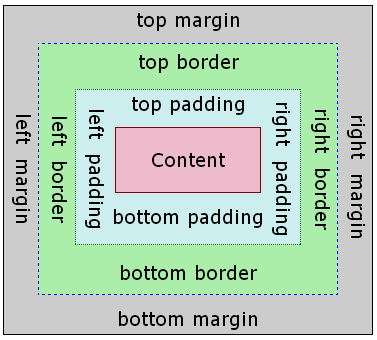
\includegraphics[width=6cm]{09/boxmodel}
\captionof{figure}{Model pudełkowy elementów strony}
\end{center}

\noindent
\textbf{!UWAGA!: }120px jest poprawne; 120 px już nie!

%%%%%%%%%%%%%%%%%%%%%%%%%%%%%%%%%%%%%%%%%%%%%%%%%%%%%%%%%%%%%%%%%%%%%%%%%%%%%%%%%%%%%%%%%%
%%% PYTANIE 150
\section{Wskaż prawdziwe stwierdzenia odnośnie poniższego fragmentu kodu PHP.}
\begin{lstlisting}[language=php, frame=single]
$fp = fopen("plik_do_blokowania", "r+");
if(flock($fp, LOCK_EX)) {
    processing();
    flock($fp, LOCK_UN);
} else {
    problem();
}
fclose($fp);
\end{lstlisting}

\noindent
{\textbf{Przykładowa odpowiedź:}}
Funkcja \textit{processing()} jest wywoływana w sekcji krytycznej.
\textbf{PRAWDA}

\vspace{0.4cm}
\noindent
\textbf{Odpowiedź:}
Brak jednoznacznej odpowiedzi.

\vspace{0.4cm}
\noindent
\textbf{Wyjaśnienie:}

\begin{enumerate}
\item 
Funkcja \textit{fopen} przyjmuje jako pierwszy argument ścieżkę do pliku, który ma zostać otwarty, a jako drugi - tryb otwarcia, jak niżej:
\begin{itemize}
\item
\textbf{r} - otwiera plik do odczytu
\item
\textbf{r+} - otwiera plik do odczytu i zapisu
\item
\textbf{w} - kasuje zawartość pliku i otwiera go do zapisu
\item
\textbf{w+} - kasuje zawartość pliku i otwiera go do zapisu i odczytu
\item
\textbf{a} - otwiera plik do dopisywania
\item
\textbf{a+} - otwiera plik do dopisywania i odczytu
\end{itemize}
Zwraca wartość liczbową identyfikującą otwarty plik.
\item
Funkcja \textit{fclose} służy do zamknięcia pliku otwartego wcześniej przez fopen. Jako argument przyjmuje liczbowy identyfikator pliku, który ma zostać zamknięty.
\item
Funkcja \textit{flock} służy do zarządzania blokowaniem dostępu do pliku jako zabezpieczenie podczas współdzielenia pliku. Zapobiega to równoczesnej modyfikacji pliku przez kilka osób/wątków.
\begin{itemize}
\item
\textbf{LOCK\_SH} - dostęp do odczytu; inne wątki mogą czytać plik, ale nie mogą zablokować go do zapisu. Zapobiega to odczytowi niepełnych danych przez inne wątki i wprowadzeniu zmian w pliku czytanym przez inne wątki.
\item
\textbf{LOCK\_EX} - dostęp do zapisu; wątek blokując plik w ten sposób ma go 'na wyłączność'. Inne wątki nie mogą go odczytać, a tym bardziej zapisać. Zapobiega wprowadzaniu zmian przez kilka wątków jednocześnie oraz odczytania niepełnych (przed edycją) danych.
\item
\textbf{LOCK\_UN} - zwolnienie blokady 
\item
\textbf{LOCK\_NB} - Gdy ustawiona, proces który natknął się na blokadę nie będzie czekał na swoją kolej. Używa się tej opcji w połączeniu, z którąś opcją blokady np. \textit{flock(\$fp, LOCK\_EX | LOCK\_NB)}. Użyta w naszym przypadku pozwoliła by na przejście bo bloku \textit{else} gdy plik jest już zablokowany, zamiast czekać na zwolnienie.\textbf{LOCK\_UN}
\end{itemize}
\textit{flock} zwraca true w przypadku sukcesu i false w przeciwnym razie.
Gdy \textit{flock} nie może uzyskać do zasobu, oczekuje na zwolnienie blokady przez inny wątek!

Funkcja \textit{flock} może przyjmować także opcjonalnie trzeci parametr. Jego wartość jest ustawiana jako 1, gdy proces zostanie zablokowany (nie uzyska dostępu do pliku). Głównie służy do sprawdzenia czy coś złego się nie wydarzyło - gdy funkcja zwraca \textbf{false}, a trzeci parametr ma wartość 0, oznacza to że wystąpił jakiś błąd, ponieważ \textit{flock} nie mógł uzyskać blokady, a jednak proces nie został wstrzymany przez już istniejącą blokadę na pliku.
\end{enumerate}


\textbf{Analiza kodu:}
\begin{enumerate}
\item
Otwieramy plik "plik\_do\_blokowania" w celu odczytu i zapisu. Identyfikator przypisujemy do zmiennej \$fp.
\item
Następnie próbujemy uzyskać dostęp do pliku w trybie exclusive.
Jeżeli plik nie został wcześniej zablokowany ani do odczytu, ani zapisu przez inny wątek - funkcja \textit{flock} zwraca \textbf{true} i blokuje plik.
\item
Wówczas wchodzimy w sekcję krytyczną gdzie aktywowana jest funkcja \textit{processing()}.
\item
Po jej wykonaniu blokada pliku jest zwalniana poprzez \textit{flock(\$fp, LOCK\_UN)}.
\item
Jeżeli plik jest odczytywany lub zapisywany przez inny wątek (został wcześniej zablokowany) funkcja \textit{flock} zwraca \textbf{false}.
Wówczas \textit{flock} oczekuje na zwolnienie blokady przez inny wątek; czeka na swoją kolej.
\item
Po wykonaniu powyższych czynności plik zostaje zamknięty.
\end{enumerate}

\noindent
\textbf{!Uwaga!: }Tak naprawdę, w tym przykładzie nie wejdziemy do bloku 'else'! (chyba, że coś złego wydarzy przy próbie blokowania)

%%%%%%%%%%%%%%%%%%%%%%%%%%%%%%%%%%%%%%%%%%%%%%%%%%%%%%%%%%%%%%%%%%%%%%%%%%%%%%%%%%%%%%%%%%
%%%% Pytanie 151
\section{Zawartość poniższego formularza przesłano do skryptu PHP. Zaznacz prawdziwe stwierdzenia.}
\begin{lstlisting}[language=html, frame=single]
<form action="skrypt.php" method="post" enctype="multipart/form-data">
    <p>
        <input type="file" name="plik"/>
        <input type="text" name="comment" />
        <input type="submit" value="wyslij" />
    </p>
</form>
\end{lstlisting}

\noindent
{\textbf{Przykładowa odpowiedź:}}
W zmiennej \textit{\$\_POST['comment']} będzie dostępna zawartość pola tekstowego.
\textbf{PRAWDA}

\vspace{0.4cm}
\noindent
\textbf{Odpowiedź:}
Brak jednoznacznej odpowiedzi.

\vspace{0.4cm}
\noindent
\textbf{Wyjaśnienie:}
Formularz php składający się z trzech elementów:
\begin{enumerate}
\item
Kontrolka do uploadu pliku. Klikając klawisz pojawi się okno eksploratora i można wybrać plik z dysku. Zmienna z nim związana nazwana została 'plik'.
\item
Pole tekstowe, umożliwiające wpisanie tekstu przez użytkownika. Pierwotnie pole tekstowe jest puste. Zmienna z nim związana nazwana została 'comment'.
\item
Klawisz zatwierdzający formularz. Po jego wciśnięciu dane z formularza zostają wysłane do skryptu 'skrypt.php' metodą POST.
\end{enumerate}

Parametr \textbf{enctype} określa w jaki sposób dane z formularza zostaną przekształcone. Może być użyty TYLKO w połączeniu z \textbf{method="POST"}.
	Możliwe wartości:
\begin{itemize}
\item
\textbf{application/x-www-form-urlencoded} - DOMYŚLNE; Wszystkie dane są przekształcane. Spacje zmieniane na +, znaki specjalne zmieniane na wartości ASCII HEX.
\item
\textbf{multipart/form-data} - żadne znaki nie są przekształcane; wymagany w przypadku użycia w formularzu kontrolki typu \textbf{'file'}
\item
\textbf{text/plain}- spacje są przekształcane na znak +, znaki specjalne nie są przekształcane
\end{itemize}

Po stronie skryptu php dostępne są wartości z tablicy asocjacyjnej \textit{\$\_POST} (pola z formularza z metodą \textbf{POST}; przy użyciu metody \textbf{GET} wartości dostępne są spod \textit{\$\_GET}) oraz \textit{\$\_FILES} (dane z kontrolki typu \textbf{file}).

\begin{itemize}
\item
\$\_POST: Array ([comment] => <tresc\_komentarza\_wpisana\_w\_polu>)
\item
\$\_FILES: Array ([plik] => Array ([name] => <nazwa\_pliku> [type] => image/png [tmp\_name] => <sciezka\_do\_pliku\_w\_tempie> [error] => 0 [size] => 38676))
\end{itemize}
Do elementów dostać się można na przykład: \textit{\$\_POST['comment']}, \textit{\$\_FILES['plik']['name']}.

Elementy formularza zgrupowane są wewnątrz znacznika akapitu (<p>).

%%%%%%%%%%%%%%%%%%%%%%%%%%%%%%%%%%%%%%%%%%%%%%%%%%%%%%%%%%%%%%%%%%%%%%%%%%%%%%%%%%%%%%%%%%
%%%% Pytanie 152
\section{Co jest efektem działania poniższego programu~w języku PHP.}
\begin{lstlisting}[language=php, frame=single]
<?php
    $wiek = array('ala'  => 12, 'ela' => 22, 'franek' => 54);
    foreach ($wiek as $k =>$w)
        echo $k.' '.$w."\n";
?>
\end{lstlisting}
{\textbf{Przykładowa odpowiedź:}}
Wygenerowanie na standardowym wyjsciu m.in. wartości komórek z tablicy  \textit{\$wiek}.
\textbf{PRAWDA}

\vspace{0.4cm}

\noindent
\textbf{Wyjaśnienie:}\\
\noindent
Tablice~w PHP działają jak mapy, mają pary kluczy wraz~z wartościami.~W związku~z tym zostanie wypisany następujący ciąg:
\begin{lstlisting}[language=html,frame=single]
  ala 12
  ela 22
  franek 54
\end{lstlisting}
\vspace{0.4cm}

%%%%%%%%%%%%%%%%%%%%%%%%%%%%%%%%%%%%%%%%%%%%%%%%%%%%%%%%%%%%%%%%%%%%%%%%%%%%%%%%%%%%%%%%%%
%%%% Pytanie 153
\section{Jak długi będzie czas wykonania poniższego programu napisanego w języku PHP?}
\noindent
\textbf{Zakłada się, że program uruchamiany jest jako aplikacja WWW tj. dostępny jest pod określonym adresem URI, a interpreter PHP uruchamiany jest przez serwer WWW.}

\begin{lstlisting}[language=php,frame=single]
<? php
    echo 'start';
    sleep(6);
?>

\end{lstlisting}
{\textbf{Przykładowa odpowiedź:}}
Dokładnie 6 sekund.
\textbf{FAŁSZ}

\vspace{0.4cm}
\noindent
\textbf{Odpowiedź:}
Dłużej niż 6 sekund.
\vspace{0.4cm}

\noindent
\textbf{Wyjaśnienie:}\\
\noindent
Wywołanie \textbf{sleep(6)} powoduje "uśpienie" programu na 6 sekund. Do tego czasu należy doliczyć także czas wykonania instrukcji \textbf{echo 'start'}, więc ogólny czas wykonania programu będzie większy niż 6 sekund. Sprawdzone za pomocą funkcji \textbf{microtime()}.

\vspace{0.4cm}
\noindent

%%%% Pytanie 154
\section{Która~z poniższych metod~w języku JavaScript zwraca element~o unikalnym identyfikatorze \textit{form}?}
\noindent
{\textbf{Przykładowa odpowiedź:}}
\begin{lstlisting}[language=html]
document.getElementByUId('form');
\end{lstlisting}
\textbf{FAŁSZ}

\vspace{0.4cm}
\noindent
\textbf{Odpowiedź:}
\begin{lstlisting}[language=html]
document.getElementById('form');
\end{lstlisting}


%%%% Pytanie 155
\section{Zaznacz prawdziwe stwierdzenia dotyczące poniższego kodu~w języku JavaScript}

\begin{lstlisting}[language=html, frame=single]
car = new Array();
car[0] = new Object();
car[0].make = 'Fiat';
car[0].vin = '123';
car[1] = new Object();
car[1].make = 'Ford';
car[1].vin = '456';

for(idx in car){
    for(prop in car [idx]){
        document.write(car[idx][prop]);
    }
}
\end{lstlisting}
\noindent
{\textbf{Przykładowa odpowiedź:}}
Na koncu dokumentu XHTML zostanie wygenerowany ciąg bajtów: \textit{makevinmakevin}.
\textbf{FAŁSZ}

\vspace{0.4cm}
\noindent
\textbf{Odpowiedź:}
Pierwsza pętla operuje po obiektach,~a druga po ich wartościach.~W związku~z tym zostanie wygenerowany ciąg znaków:\\ \textit{Fiat123Ford456}~w miejscu,~w którym został wstawiony kod.

\vspace{0.4cm}

\noindent
\textbf{UWAGA:} Kolejność iteracji po właściwościach obiektów (a nawet po tablicy) może być zależna od samej przeglądarki, co mogło by wpływać na odpowiedź.

%%%% Pytanie 156
\section{Zaznacz prawdziwe stwierdzenia dotyczące poniższego kodu w języku JavaScript.}
\begin{lstlisting}
function updateAjax() {
    xmlhttp = new XMLHttpRequest();
    xmlhttp.onreadystatechange = function() {
        if (xmlhttp.readyState == 4 && xmlhttp.status == 200) {
            document.getElementById("stime").innerHTML = xmlhttp.responseText;
        }
    }
    xmlhttp.open("GET", "date.php", true);
    xmlhttp.send();
    window.setTimeout("updateAjax()", 1000);
}
window.setTimeout("updateTime(); updateAjax();", 5000);
\end{lstlisting}

\noindent
{\textbf{Przykładowa odpowiedź:}}
Komunikacja AJAX rozpocznie się po 5000 sekund od zinterpretowania powyzszego kodu.
\textbf{FAŁSZ}

\vspace{0.4cm}
\noindent
\textbf{Odpowiedź:}
Komunikacja AJAX rozpocznie się po 5000 milisekund (czyli po 5 sekundach) od zinterpretowania powyższego kodu.

\vspace{0.4cm}
\noindent
\textbf{Wyjaśnienie:}

\begin{itemize}
\item{Event \textbf{XMLHttpRequest.onreadystatechange} jest triggerowany za każdym razem, gdy
\textbf{XMLHttpRequest.readyState} się zmienia}

\item{\textbf{XMLHttpRequest.readyState == 4} oznacza, że wysłany przez nas request został zakończony.}

\item{\textbf{XMLHttpRequest.status == 200 } (HTTP status 200) oznacza, że nasz request został przetworzony poprawnie}

\item{\textbf{XMLHttpRequest.responseText} jest odpowiedzią serwera na nasz request. W przypadku powyższego kodu elementowi \textbf{na naszej stronie} o id == 'stime' zostanie przypisana odpowiedź serwera.} 

\item{Funkcja \textbf{XMLHttpRequest.open(method,url,async)} określa typ requestu jaki zostanie wysłany. }

\item{\textbf{window.setTimeout(function, milliseconds)} powoduje pojedyncze uruchomienie funkcji (jak widać w powyższym kodzie może ich być kilka) określonej przez parametr \textbf{function} po odczekaniu czasu określonego przez parametr \textbf{miliseconds}.}

\end{itemize}
Komunikacja AJAX rozpocznie się po 5 sekundach od zinterpretowania kodu. Następnie funkcja \textbf{updateAjax()} będzie wywoływana co jedną sekundę (sama ustawia sobie timeout).


\vspace{0.4cm}
\noindent

%%%% Pytanie 157

\answer{Dany jest dokument XML oraz odpowiednie DTD. Zaznacz prawdziwe stwierdzenia.}
{Funkcjonalność DTD może być zastąpiona przez XML Schema.}{T}
{Patrz poniżej}
{\\}

\vspace{0.2cm}
\noindent
\begin{description}
\item[DTD] rodzaj dokumentu definiujący formalną strukturę dokumentów XML, HTML, XHTML lub innych
 pochodzących z rodziny SGML lub XML. Definicje DTD mogą być zawarte w pliku dokumentu, którego strukturę definiują, przeważnie jednak zapisane są w osobnym pliku tekstowym, co pozwala na zastosowanie tego samego DTD dla wielu dokumentów.\\

\item[XMLSchema] - opracowany przez W3C standard służący do definiowania struktury dokumentu XML. XML Schema stanowi alternatywę dla DTD, przy czym posiada znacznie większe możliwości. XML Schema jest strukturą XML, w odróżnieniu od DTD nie będącego częścią standardu XML. Dokumenty zawierające definicje XML Schema zapisuje się zwykle w plikach z rozszerzeniem .xsd (od XML Schema Definition).
\end{description}

\textbf{Funkcjonalność DTD może zostać zastąpiona przez XMLSchema. Należy jednak pamiętać, że składnia XMLSchema sama w sobie jest zazwyczaj definiowana przez DTD.}\\
\\
Dokładniejszy opis różnic pomiędzy DTD a XMLSchema oraz ich składnię można podejrzeć tutaj:\\
http://www.sitepoint.com/xml-dtds-xml-schema/

\vspace{0.2cm}
\noindent \textbf {Zdania prawdziwe na temat XML, DTD, XML Schema:} 
\begin{itemize}
	\item{XML można zwalidować przy pomocy DTD}
	\item{XML musi zawierać deklarację (prolog) i jeden element główny}
    \item{XML ma strukturę drzewiastą}
    \item{XML nie ma żadnych predefiniowanych znaczników}
    \item{obowiązkowe atrybuty znaczników muszą być zdefiniowane w DTD}
    \item{jeśli chcemy zdeklarować encję to robimy to w DTD}
    \item{aby można było mówić o poprawnym strukturalnie dokumencie XML musi być zdefiniowane DTD, dokument musi być dobrze sformułowany, zawierać prawidłowe odwołanie do TD i być z nim zgodny}
    \item{DTD może być załączone w dokumencie XML, dostępne w systemie, dostępne przez URL}
    \item{DTD może zawierać deklaracje}
    \begin{itemize}
    	\item{<!ELEMENT nazwa (skladnia)>}
    	\item{<!ATTLIST atr1 typ wartosc atr2 typ wartosc>}
        \item{<!ENTITY nazwa tresc>}
	\end{itemize}
    \item{DTD może być wewnętrzne i zewnętrzne (dołączane w osobnym pliku)}
    \item{DTD zewnętrzne i wewnętrzne można łączyć}
    \item{DTD jest zapisywany w osobnym języku (opartym o BNF)}
    \item{XML Schema są zapisywane w XML}
    \item{XML Schema mają większe możliwości rozszerzenia i rozbudowy}
    
    
\end{itemize}    